\renewcommand{\captiontitle}{空间变换网络模块}
\begin{figure}
\begin{center}

\begin{tikzpicture}
\node [anchor=south west] (image) at (0,0) {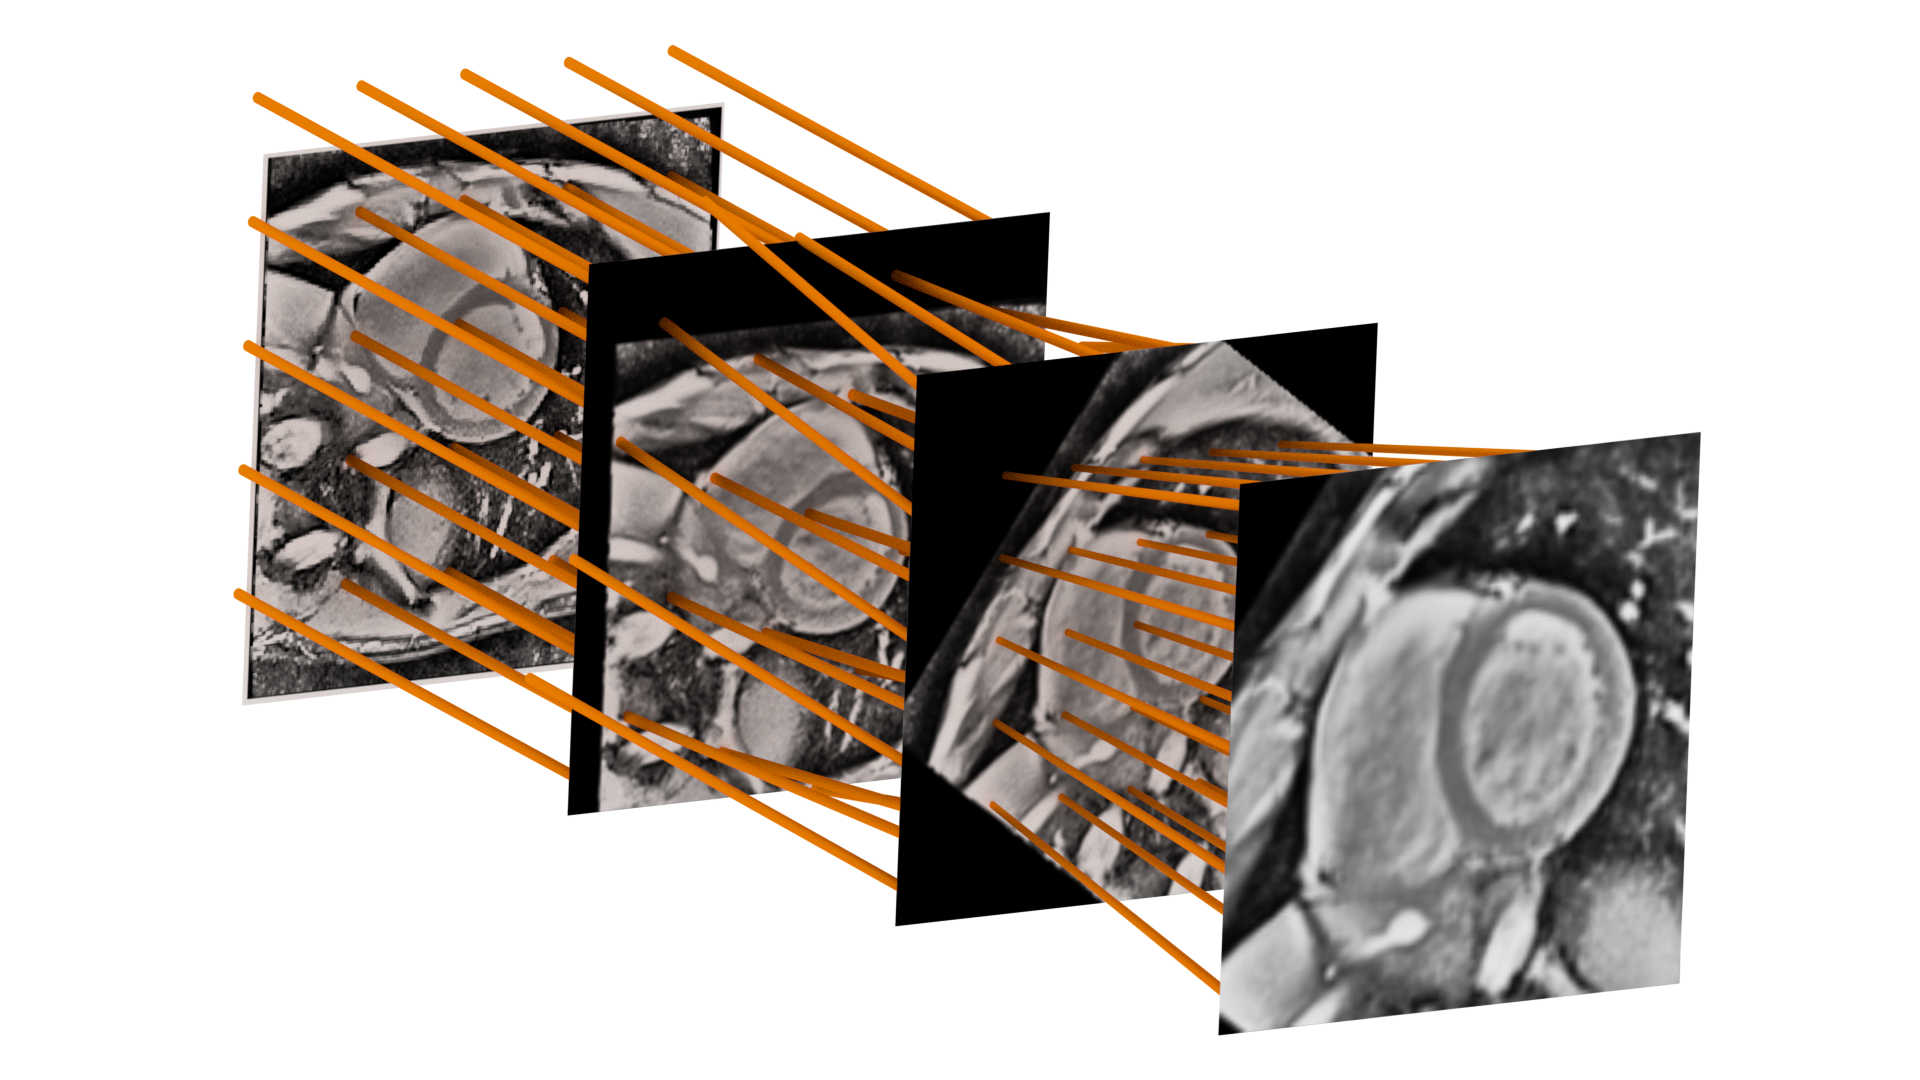
\includegraphics[width=0.5\textwidth]{./data/sampler.png}};
\draw [decorate,decoration={brace,amplitude=10pt},xshift=0pt,yshift=0pt](2.8,1.317) -- (1.25,1.85) node [black,midway,xshift=-0.3cm,yshift=-0.7cm] {\footnotesize $\image_2 = \trans(\image, T)$};
\draw [decorate,decoration={brace,amplitude=10pt},xshift=0pt,yshift=0pt](4.35,0.783) -- (2.8,1.317) node [black,midway,xshift=-0.3cm,yshift=-0.7cm] {\footnotesize $\image_3 = \trans(\image_2, R)$};
\draw [decorate,decoration={brace,amplitude=10pt},xshift=0pt,yshift=0pt](5.9,0.25) -- (4.35,0.783) node [black,midway,xshift=-0.3cm,yshift=-0.7cm] {\footnotesize $\trans(\image_3, S)$};
\end{tikzpicture}

\caption[\captiontitle]{\captiontitle{}.请注意,在实际的实现中,所有的变换都是相对于输入图像 $\image$ (即 $\trans(\image, T)$,$\trans(\image, RT)$和$\trans(\image, SRT)$)的变换;我们在此处只是为了清晰地说明这是连续处理的步骤.}
\label{fig:stn-module}
\end{center}
\end{figure}

